\documentclass[12pt,a4paper]{article}

\usepackage[utf8]{inputenc}
\usepackage[spanish,activeacute]{babel}
\selectlanguage{spanish}
\usepackage{amsmath}
\usepackage{amsfonts}
\usepackage{amssymb}
\usepackage[font=scriptsize,labelfont=bf]{caption}

\usepackage{multirow}
\usepackage{graphicx}

\usepackage[left=4cm,right=4cm,top=4cm,bottom=4cm]{geometry}
\usepackage{listings} 
\usepackage{tikz}
\usepackage{enumerate}

\usetikzlibrary{arrows}


\newlength{\margen}
\setlength{\margen}{\paperwidth}
\addtolength{\margen}{-\textwidth}
\setlength{\margen}{0.5\margen}
\addtolength{\margen}{-1in}
\setlength{\oddsidemargin}{\margen}
\setlength{\evensidemargin}{\margen}

\usepackage{hyperref}


\title{Sistemas Distribuidos de Procesamiento de Datos\\Práctica Hadoop MapReduce}
\author{\\Jon Kobeaga Urriolabeitia\\ José Vicente Mellado \\Universidad Rey Juan Carlos}

\begin{document}

\maketitle
\hrule
\tableofcontents
\newpage
\section{Introducción}
En este documento se explicarán los pasos, el código, las conclusiones y los problemas tenidos a la hora de hacer el análisis de sentimientos de los estados de Estados Unidos. 

Para llevar acabo dicho análisis se ha utilizado un fichero, llamado \textit{AFIN-en-165}, creado por Finn Årup Nielsen entre los años 2009 y 2015, que nos indica la felicidad que nos aporta cada palabra. La lista fue creada a mano y a cada palabra le corresponde un número entero entre [-5,5]. Un valor de 5 representa felicidad máxima y un valor de -5 representa tristeza absoluta.
Dicho archivo se puede encontrar en el repositorio oficial del proyecto: \url{https://github.com/fnielsen/afinn/blob/master/afinn/data/AFINN-en-165.txt}.


\section{Descripción del código}

En este apartado explicaremos el código utilizado para hacer el análisis de sentimientos. Se ha dividido en tres fases principales:

\begin{enumerate}
\item Obtención de los datos.
\item Análisis de los datos.
\item Representación de los resultados.
\end{enumerate}

\subsection{Obtención de los datos}
Se ha levantado una instancia de EC2 de Amazon Web Services para obtener los tweets. Los datos conseguidos se han guardado en formato JSON y para su obtención se han utilizado dos criterios diferentes:

Por una parte, se ha descargado el 1\% de todos los tweets que se generan en el momento, sin tener en cuenta la localización ni el idioma. De esta forma se han descargado 1,7GB.\\
Por otra parte, se ha hecho un filtrado para descargar los tweets, obteniendo sólo los tweets en inglés y de Estados Unidos. Para ello, hemos hecho uso de los métodos que ofrece la API de Twitter indicando, a través de distintos parámetros, el área que nos interesa de tal manera que se recuperan únicamente los tweets generados entre Canadá y México. 
El estado se guarda en el campo ``usa\_state''. Además, como cada tweet tiene mucha información que no se iba a utilizar posteriormente, sólo hemos guardado los campos que nos interesan con el objetivo de que ocupar el menor espacio posible. De esta forma se han descargado 300MB y 500.000 tweets.\\
En total, se ha trabajado con un fichero de 2GB y 829.576 tweets.


\subsection{Análisis de Resultados}

El análisis de resultados consiste en dos scripts: \textit{mapreduce\_jobs/tweets.py} en el que está codificado en sí el objetivo de la práctica utilizando el modelo MapReduce y el otro, \textit{mapreduce\_jobs/word\_utils.py}, con métodos que sirven para facilitar el trabajo de las funciones principales. 

Como era un requisito codificar una solución en Python siguiendo el modelo MapReduce, hemos optado por utilizar la librería MRJob explicada en clase. MRJob es un \textit{framework} que permite escribir y desplegar fácilmente \textit{jobs} MapReduce en diferentes plataformas (AWS, Google Cloud y clústeres Hadoop).

MRJob ofrece una manera de dividir el objetivo global en subobjetivos llamados \textit{steps} (pasos). A continuación, se van a detallar los dos pasos de los que se compone nuestra solución.

\subsubsection{Primer paso}
En este primer paso se ejecutan el mapper, el combiner y el reducer. Para que se pueda ejecutar el mapper, se necesita tener un diccionario de las palabras y su correspondiente nivel de felicidad. Este diccionario se crea a través del archivo \texttt{AFINN-en-165.txt}. Además, si alguna palabra no está en el diccionario se ha considerado que la felicidad que aporta es nula. Ahora, explicaremos en qué consiste cada función:

\begin{itemize}
\item \textbf{Mapper:} Se lee cada tweet y lo primero que se filtra es el idioma, nos quedamos con los tweets en inglés. Después, dependiendo del criterio utilizado para descargar el tweet, hay diferentes campos que nos indican la localización. Si el tweet descargado ya ha sido filtrado, el campo que nos indica el estado es ``usa\_state''. Si el tweet no ha sido filtrado, hay dos campos que nos indican su localización: ``user''$\rightarrow$``location'' y ``place''$\rightarrow$ ``country''. Se ha utilizado la libreria \texttt{us} para obtener el estado partiendo de la información de los campos.\\

Después se ha obtenido el texto del tweet, que nos indica el campo ``text''. Debido a que cada palabra del fichero \textit{AFIN-en-165} está en minúscula, hemos pasado cada palabra a minúscula y solamente hemos cogido los caracteres del alfabeto inglés y ``\#'' que hace referencia a los hashtags.\\

Una vez se tienen las palabras del tweet en ambos casos, tanto si la palabra es hashtag o no se emitirá un par \textit{(clave, valor)}. Si la palabra es un hashtag, ese par tendrá como clave el hashtag y como valor 1 (\textit{(\#hashtag, 1)}). En caso contrario, se emitirá un par que tendrá como clave el estado desde el que se escribió el tweet que contiene esa palabra y como valor la puntuación de sentimiento de esa palabra (\textit{(estado, valoraciónDeLaPalabra)}).

\item \textbf{Combiner:} Este paso se utiliza para simplificar el trabajo en el reducer. Suma el valor de los hashtags y los estados y los envía como \textit{(\#hashtag o estado, valor)}.

\item \textbf{Reducer:} Suma el valor de los hashtags y de los estados resultando una lista de pares clave-valor. Para cada tupla clave-valor se diferencia si se trata de un hashtag o de un estado. Si se trata de un hashtag la tupla \textit{(valor, \#hashtag)} se guarda de la siguiente manera: (\textit{("hashtag", (valor, \#hashtag))}).Si se trata de un estado se almacena así (\textit{("state", (valoraciónDeLaPalabra, estado))}).

Hemos decidido separar los resultados por una nueva clave en función de si es hashtag o estado porque esa colección de claves-valor la usaremos posteriormente en un reducer. Si los resultados están agrupados por claves, al utilizarlo como entrada en un reducer, el procesamiento de los mismos se podrá paralelizar porque el trabajo a realizar sobre cada par es independiente de otros con distinta clave.

\subsubsection{Segundo paso}

En este segundo paso, se obtienen  la felicidad de cada estado, el estado más feliz y los diez hashtags más utilizados. Todo esto se realiza en un único reducer.\\

Se crean dos diccionarios por separado, uno con todos los estados y su respectiva felicidad y otro con todos los hashtags y el número de veces que se han utilizado. Después se ordenan los diccionarios y se coge el estado más feliz y los diez hashtags más comunes.

Por pantalla se muestra primero el top 10 de hashtags más usados, después todos los estados de los Estados Unidos de América con su valoración de felicidad y finalmente el estado que mayor valoración ha obtenido (el más feliz).

En el archivo \textit{report/output.txt} se puede ver la salida del programa con los datos que hemos usado.
\end{itemize}

Al final de este documento, en el Anexo, se encuentra un diagrama con el flujo de datos entre los diferentes steps, Figura \ref{diagrama}.

\subsection{Representación de los Datos}
Los resultados obtenidos se han representado en un mapa de colores. El script para pintar el coloreado cada estado se ha obtenido del Github de Matplotlib 	\url{https://github.com/matplotlib/basemap/blob/master/examples/fillstates.py}.\\
Cada estado se ha pintado de un color dependiendo de su nivel de felicidad. Se han utilizado \texttt{ShapeFiles}, para dibujar los estados con sus respectivas fronteras. Para representar los resultados, se ha utilizado la librería \texttt{Basemap}.\\

Se ha escalado la felicidad de cada estado para que a la hora de pintar no haya diferencias grandes. La fórmula a utilizar para el escalado ha sido la siguiente:
$$hap_{estado}=1-\displaystyle \sqrt{\dfrac{hap-hap_{min}}{hap_{max}-hap_{min}}}$$

donde \textit{hap} indica la felicidad del estado y $hap_{max}\ \text{,}\ hap_{min}$ son el valor máximo y mínimo de felicidad.
El estado más feliz se pinta de azul y el menos feliz de un color amarillo-verdoso. El script encargado de la representación es \textit{report/paint\_states.py}. 


\begin{figure}[h]
\centering
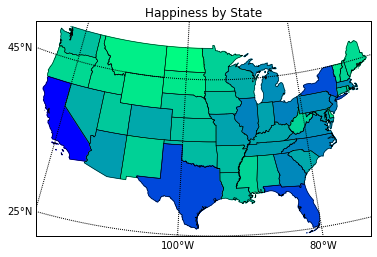
\includegraphics[scale=1]{happiness.png}
\caption{Gráfico que representa la felicidad de cada estado.}
\label{hap-stat}
\end{figure}

Como se ve en la Figura \ref{hap-stat}, con los datos que tenemos, el estado más feliz es claramente California, pero Texas, Florida y New York, también son estados muy felices. En cambio, Dakota del Norte, Dakota de Sur, Montana y Vermont son los estados más tristes según los datos que tenemos. Los estados más felices coinciden con los estados más poblados  y los menos felices con los menos poblados. Este resultado puede ser a causa del número de tweets recogidos en cada estado, es decir, cuando mayor es la población mayor es el número de tweets y por tanto, mayor es la felicidad.

\section{Diferentes Formas de Ejecución}

Se ha ejecutado de cinco formas diferentes:
\begin{enumerate}
\item Local: \texttt{python \_\_init\_\_.py ../assets/tweets.json \\--file ../assets/AFINN-en-165.txt} Tiempo: 1min 30 seg
\item Horton local: \texttt{python \_\_init\_\_.py -r inline ../assets/tweets.json  --file ../assets/AFINN-en-165.txt } Tiempo: 2mins 15 seg
\item Horton cluster Hadoop: \texttt{python \_\_init\_\_.py -r local ../assets/tweets.json  \\ --file ../assets/AFINN-en-165.txt} Tiempo: 2mins 15 seg
\item HDFS Hadoop: \texttt{python \_\_init\_\_.py -r hadoop \\ hdfs:///tweets/tweets.json1 --hadoop-streaming-jar /usr/hdp/2.5.0.0-1245/hadoop-mapreduce/hadoop-streaming.jar}
\item EMR : \texttt{python \_\_init\_\_.py -r emr s3://urjc.datascience.jon/tweets\\/tweets1.json -c ./tweets\_mrjob.conf \\--output-dir=s3://urjc.datascience.jon/tweets/Resultados}
\end{enumerate}

En el caso de EMR, la opción -c permite elegir un archivo de configuración que usará MRJob internamente para desplegar la aplicación en Elastic MapReduce. En el archivo \textit{tweets\_mrjob.conf} se encuentra la configuración necesaria para que nuestra solución propuesta funcione correctamente.

\section{Evaluación de Escalabilidad y Elasticidad}

Cuando se ejecuta el programa en un cluster de Hadoop simulado en nuestro ordenador local, el tiempo  utilizado no supera los dos minutos y medio. En cambio, para ejecutarlo en EMR el tiempo utilizado es de 5 minutos y medio con 5 procesadores. A este tiempo hay que añadirle la demora que supone levantar las distincias instancias para el clúster. 

\begin{figure}[h]
\centering
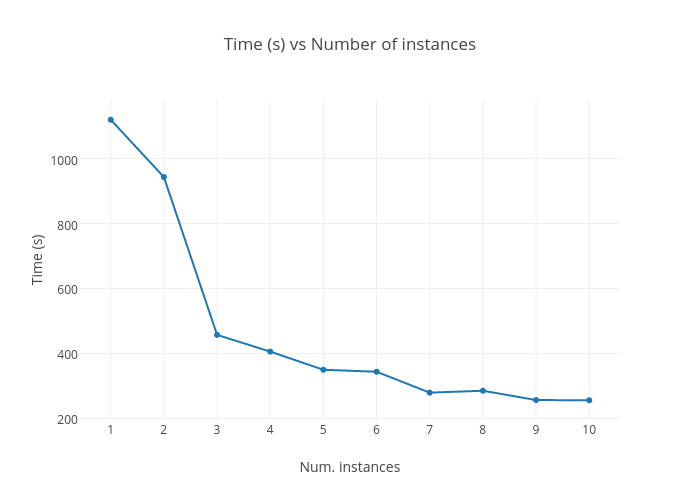
\includegraphics[scale=0.5]{plot.png}
\caption{Time (s) vs Number of instances con un fichero de 1.7GB, instancias de tipo m1.medium}
\label{tiempos}
\end{figure}

En la Figura \ref{tiempos} se pueden apreciar las consecuencias de la Ley de Amdahl ya que cuando se realiza la ejecución con 7 instancias el disminución de tiempo es muy pequeño en comparación con ejecuciones anteriores. Esto sucede porque a partir de siete procesadores ha llegado el momento en el que no se puede paralelizar más. Si quisiéramos que fuera más efectivo tendríamos que explotar más el algoritmo.\\

Sin embargo, hay que tener en cuenta la ley de Gustafson, ya que muchas veces la paralelización no se utiliza para realizar una tarea más rápido, sino para abordar problemas de mayor tamaño. Es decir, en nuestro caso, un fichero de 1.7GB sin paralelizar se ha ejecutado en dos minutos y medio, y paralelizando en cinco minutos y medio, pero, si tuviéramos un fichero lo suficientemente grande, con la paralelización el tiempo de ejecución sería menor. Además, si pusiéramos más procesadores el tiempo de ejecución se reduciría, pero únicamente el del mapper y el del combiner, porque se dividiría más el trabajo. En cambio, el tiempo empleado en el reducer seguiría siendo el mismo, porque, al tener únicamente dos claves diferentes, no es posible dividir más el trabajo.\\

La solución (modelo MapReduce) que estamos aplicando al problema puede tardar más que en nuestro computador doméstico, pero a cambio nos proporciona una fácil escalabilidad en caso de que el problema se hiciera más grande y necesitara más recursos.

\section{Comentarios Personales}

En cuanto a aspectos técnicos, hemos usado la librería \textit{ujson} que es más rápida que la librería \textit{json} que Python contiene por defecto. Hemos intentado seguir al máximo la guía de estilos PEP 8 y en la medida de lo posible también la guía PEP 20, además de seguir una estructura recomendada para proyectos Python y documentar la mayoría de métodos usando docstrings.
Como herramienta de control de versiones se ha usado Git y este proyecto se encuentra en un repositorio de GitHub en el siguiente enlace: \url{https://github.com/jvicentem/tweets-sentiment-analysis}.\\

Uno de los problemas principales que hemos tenido ha sido en la obtención de datos. Además de que de todos los tweets descargados muchos no eran útiles para nuestro análisis, porque no estaban en inglés ni eran de Estados Unidos, otros carecían de localización o se descargaron erróneamente (por ejemplo, algunos tweets se descargaron sin los ``:'' que identifican a cada campo). Por tanto, pensamos que es mejor hacer el filtrado antes descargar los tweets (teniendo en cuenta que sabemos lo que necesitamos y lo que vamos a hacer con los datos), para así, tener únicamente los tweets necesarios y ocupar menos espacio.\\

Otro de los problemas que hemos tenido, ha sido con el nombre de los bucket, que para ejecutar el MRJob no pueden tener ningún ``.'' en el nombre. Afortunadamente hemos solventado esto añadiendo un par de líneas justo después de la importación de bibliotecas en \textit{tweets.py}\\


Por otra parte, para un análisis más correcto, se debería de recoger un número parecido de tweets por estado, porque, viendo los resultados obtenidos, cuando mayor es el número de tweets mayor es la felicidad, por lo que no se refleja bien la felicidad de cada estado.\\
Además, como una única palabra, por sí sola, puede ser un poco ambigua, otra de las mejoras que se pueden hacer es analizar tuplas y tripletas de palabras para tener en cuenta el contexto.\\

\newpage
\section{Anexo}
\begin{figure}[htp]

\makebox[\textwidth][c]{\includegraphics[width=1.55\textwidth]{MapReduceFlow.png}}
\caption{Flujo entre los diferentes steps}
\label{diagrama}
\end{figure}


\end{document}